\documentclass[11pt, oneside]{article}   	
\usepackage{geometry}                		
\geometry{letterpaper, margin=1in}              
\usepackage{graphicx}					
\usepackage{amssymb}
\usepackage{amsmath}
\usepackage{booktabs}
\usepackage{listings}
\usepackage{color}
\usepackage{multirow}
\usepackage{siunitx}
\usepackage[ruled,vlined]{algorithm2e}

\definecolor{dkgreen}{rgb}{0,0.6,0}
\definecolor{gray}{rgb}{0.5,0.5,0.5}
\definecolor{mauve}{rgb}{0.58,0,0.82}

\lstset{frame=tb,
   language=[90]Fortran,
   aboveskip=3mm,
   belowskip=3mm,
   showstringspaces=false,
   columns=flexible,
   basicstyle={\small\ttfamily},
   numbers=none,
   numberstyle=\tiny\color{gray},
   keywordstyle=\color{blue},
   commentstyle=\color{dkgreen},
   stringstyle=\color{mauve},
   breaklines=true,
   breakatwhitespace=true
   tabsize=3
   }


\title{MCSC 6030G : High Performance Computing \\ Assignment 3: Langevin Dynamics of Interacting Particles}
\author{Parikshit Bajpai \\ 100693928}
\date{}							% Activate to display a given date or no date

\begin{document}
\maketitle

\section{Introduction}
In 1908, Paul Langevin successfully applied Newtonian dynamics to a Brownian particle to come up with what is now called as the 'Langevin equation', the stochastic physics equivalent to the second law of motion (\(F=ma\)). This stochastic differential equation is applicable to continous Markov processes and shows that the root mean square dispalcement of a Brownian particle is proportional to the square root of time. The Langevin equation contains both viscous and random forces with the two forces related by the fluctuation-dissipation theorem. In the modern notation, Langevin equation takes the following form:     
  \begin{equation} \label{Langevin}
    m\,dv = - \gamma\,v\,dt + \sqrt{dt}\,c\,\eta(t) 
  \end{equation}
  where the velocity of the particle, \(v \in \mathbb{R}^2\) in a two-dimensional space, \(\gamma\)  denotes the viscosity contribution of the force, and the random force variable \(\eta\) is drawn from a standard normal distribution. The random force  coefficient equals, from the fluctuation-dissipation theorem, \(c = \sqrt{2 \gamma k_B T}\), where \(k_B\) is the Boltzmann constant and T is the temperature.

  In Langevin dynamics, at short time scales, i.e. \(t \ll \tau_p \), where \(\tau_p =  m / \gamma \) is the momentum relaxation time of particles, the dynamics of a Brownian particle is dominated by its inertia, and, the motion is this region is termed as \textit{ballistic Brownian motion}. At larger time scales, i.e.  \(t \gg  \tau_p\), \textit{diffusive Brownian motion} is observed. When the particles are constrained in a box, we observe a third region beyond the diffusive region. In this region the RMS displacement saturates and we observe a plateau and a constant RMS displacement.
  
\section{Methodology}
   \subsection{Objective}
In the present study, Langevin dynamics studied in the previous assignment has been further analysed by including interaction forces between the particles and implementing domain decomposition and parallelisation. The objective of this study is to analyze the Brownian motion of interacting particles with domain decomposition and multi-threading, and, to study the impact of model parameters on the efficiency of parallelization.

\subsection{Machine Configuration}
The initial computations for the present study were performed on the local machine followed by detailed study on HPC systems accessible through \textit{Compute Canada}.
      \subsubsection{Local Machine}
        \textbf{Manufacturer \& Model}: Lenovo ThinkPad Yoga 370\\
	\textbf{Processor}: Intel Core i5 -7200U (2 physical cores, 2 hyperthreads)\\
	\textbf{Clock Rate}:  2.50 GHz\\
	\textbf{RAM}:  16 GB\\
	\textbf{Operating System}: Ubuntu 18.04\\

       \subsubsection{GRAHAM Cluster}
        \textbf{Manufacturer}: Huawei\\
	\textbf{Processor}: Intel E5-2683 v4 (Broadwell) (Total 36160 cores, maximum 32 cores used in the study)\\
	\textbf{Clock Rate}:  2.10 GHz\\
	\textbf{RAM}:  Node specific\\
	\textbf{Operating System}: CentOS 7\

	
\subsection{Implementation}
The Langevin equation was discretised using the Velocity Verlet algorithm, which is similar to the Leapfrog method, except that the velocity and position are calculated at the same value of the time variable. The mathematical formulation of the algorithm is shown below.
\begin{equation}
  \begin{split}
    \mathbf{x}(t + \Delta t) &= \mathbf{x}(t) +  \mathbf{v}(t)\Delta t + \frac{1}{2} \mathbf{a}(t) \Delta t^2 \\
    \mathbf{v}(t + \Delta t) &= \mathbf{v}(t) + \frac{\mathbf{a}(t) + \mathbf{a}(t+\Delta t)}{2} \Delta t \\
  \end{split}
\end{equation}

While an implementation of the above algorithm essentially involves computing forces (which manifest themselves in the code in form of accelerations) and updating velocities and positions at each time step, additional book-keeping tasks must be performed in order to include domain decomposition.

The principle behind domain decomposition is reducing the computation time by avoiding operations whose results are a-priori known. It has been well established that the interaction forces between particles at a distance larger than a critical distance, $r_c$, are effectively zero. By selecting a suitable sector size, $\text{\textit{Domain Width}} \geq R_c$, the number of interactions to be computed can be minimized to interactions between particles in the same and surrounding sectors, therby resulting in a decrease in wallclock times. Furthermore, each sector can then, at least in theory, be alloted to a separated thread in order to implement multi-threading. The overheads in domain decomposition arise from the requirement to maintain neighbour lists and to account for the particles and updating their sectors at each time step.

In the present work, reflecting boundary conditions have been implemented along with the decomposition of domain into $D \times D$ subdomains/sectors. The following pseudo-codes exhibit the algorithms required to develop a Langevin dynamics code for interacting particles with reflecting boundary conditions and domain decomposition.

\begin{algorithm}
  \DontPrintSemicolon
  \KwData{Number of particles ($N$), Number of rows and columns ($d$)}
  \KwResult{Compute RMS displacement and trajectories}
  Allocate and initialize all variables\;
  Create neighbour list\;
  Initialize particles and perform ordering\;
  \While{$t < t_{max}$}{
    Update half-step velocities $\vec v_h (t + \Delta t/2) \leftarrow \vec v(t) + 0.5 \vec a \Delta t$\;
    Update particle positions $\vec x (t+dt) \leftarrow \vec x (t) + \vec v_h (t+\Delta t /2) \Delta t$\;
    Impose reflecting boundary conditions\;
    Reorder particles according to sector\;
    Compute random forces acting on particle and update particle acceleration $\vec a$\;
    \For{Sector $S1 = 0,1,\cdots,d^2-1$}{
      \For{Each particle $i$ in sector $S1$}{
        \For{All neighbours $S2$ of sector $S1$}{
          \For{Each particle $j$ in sector $S2$}{
            Compute distance between particles $i$ and $j$\;
            \If{Distance between $i$ and $j$ $<$ Critical distance $r_C$}{
              Compute interaction force $\vec F_i$\;
              Update particle acceleration $\vec a_i \leftarrow \vec a_i + {\vec F_i}/m$\;
            }
          }
        }
      }
    }
    Update velocities $\vec v (t + dt) \leftarrow \vec v_h(t + \Delta t/2) + 0.5 \vec a \Delta t$\;
    Update time $t = t + \Delta t$\;
    Write particle position $\vec x$ to 'Trajectories'\;
    Write RMS displacement $\sqrt{\frac{\sum_{i=1}^{N}(\vec x - \vec x_0)^2}{N}}$ to 'Means'\;
  }
  \caption{Main}
\end{algorithm}

\begin{algorithm}
  \DontPrintSemicolon
  \KwData{Particle position (\(\vec x = \left< x, y \right>\)), Particle velocity (\(\vec u = \left< u_x, u_y \right>\)), Particle acceleration (\(\vec a = \left< a_x, a_y \right>\))}
  \KwResult{Set physical parameters and random initial position and velocity of particles}
      Initialize physical parameters \\
      \For{Particle $i = 1,2,\cdots,N$}{
        $x_i \leftarrow \text{Uniform random number} \in (-L/2 , L/2)$ \\
        $y_i \leftarrow \text{Uniform random number} \in (-L/2 , L/2)$ \\
        $u_{x_i} \leftarrow \text{Normal random number} \in \mathcal{N}(0, \, \frac{K_B T}{m})$ \\
        $u_{y_i} \leftarrow \text{Normal random number} \in \mathcal{N}(0, \, \frac{K_B T}{m})$ \\
        $a_{x_i} \leftarrow 0$ \\
        $a_{y_i} \leftarrow 0$
      }
   \caption{Initialization}
\end{algorithm}

\begin{algorithm}
  \DontPrintSemicolon
  \KwData{Particle position (\(\vec x = \left< x, y \right>\)), Particle velocity (\(\vec u = \left< u_x, u_y \right>\)), Box length ($L$)}
  \KwResult{Updates particle position and velocity if outside the box}
      \For{$i = 1,2,\cdots,N$}{
        \If{$x_i < -L/2$}{
          $x_i \leftarrow -L - x_i$;
          \\$u_{x_i} \leftarrow -u_{x_i}$;
        }
        \If{$x_i > L/2$}{
          $x_i \leftarrow L - x_i$;
          \\$u_{x_i} \leftarrow -u_{x_i}$;
        }
        \If{$y_i < -L/2$}{
          $y_i \leftarrow -L - y_i$;
          \\$u_{y_i} \leftarrow -u_{y_i}$;
        }
        \If{$y_i > L/2$}{
          $y_i \leftarrow L - y_i$;
          \\$u_{y_i} \leftarrow -u_{y_i}$;
        }
      }
    \caption{Reflecting Boundary Conditions}
  \end{algorithm}

\begin{algorithm}
  \DontPrintSemicolon
  \KwData{Particle position (\(\vec x = \left< x, y \right>\))}
  \KwResult{Sector indices and number of particles in each sector}
  \For{Particle $i = 1,2,\cdots,N$}{
    \If{Particle within domain ($-L/2 \leq x \leq L/2$ \textbf {and} $-L/2 \leq y \leq L/2$)}{
      Assign sector to the particle; \\
      Number of particles in sector $\leftarrow$ Number of particles in sector + 1;
    }
     \Else{
      Put the particle in garbage bin; \\
      Number of particles in garbage $\leftarrow$ Number of particles in garbage + 1;
     }
  }
  \caption{Assign particle sectors}
\end{algorithm}

\begin{algorithm}
  \DontPrintSemicolon
  \KwData{Particle position (\(\vec x = \left< x, y \right>\))), Particle velocity (\(\vec u = \left< u_x, u_y \right>\))}
  \KwResult{Particles ordered according to the sector they are in.}
  \For{Particle $i = 1,2,\cdots,N$}{
    Sort the particles according to their sector.
  }
  \caption{Ordered list of particles}
\end{algorithm}

\begin{algorithm}
  \DontPrintSemicolon
  \KwData{Neighbour list}
  \KwResult{List of neighbours of each sector}
  \For{Sector $k = 1,2,\cdots,d^2-1$}{
    \For{All surrounding sectors}{
      \If{Valid sector}{
        Add to neighbour list
      }
    }
  }
  \caption{Neighbour list}
\end{algorithm}

    
    


\subsection{Computational Experiments}
The simulation of Brownian motion depends on a number of factors, both physical and computational. These parameters not only affect the observed behaviour but also the computational times as discussed in the following paragraphs.

The number of particles, $N$, is the most important factor affecting the computations and wallclock times. As seen above, the wallclock times for the case without domain decomposition are proportional to $N^2$ and therefore if we increase the number of particles in the system by 2, we will observe an increase in the wall times by a factor of 4. In order to study the impact of the other parameters, we can then fix the number of particles in the system. However, while doing this, we must ensure that the number of particles is not too large or too small to result in a too dense or too sparse system.

The particle density in the box affects the Brownian motion itself and the  observed regions of the RMS displacements. As already seen in the previous assignment, if the particle density is too large, we'll lose the diffusive Brownian motion, and, owing to the large number of interactions, the diffusive region might not be computationally resolved and a direct transition from ballistic to saturation region will be observed. The particle density in the box is itself a function of the number of particle in the domain, $N$, and the length of the box, $L$. For a fixed number of particles in the domain, we want to keep the size of the box as large as possible. However, it must also be ensured that we do not make the box too large, and hence the particle density too sparse, therby imposing an upper limit on the box size.

The wallclock times for the Langevin dynamics problem depend on the maximum time of simulation, $t_{max}$, and the time-steps, $\Delta t$, used in the simulations. While the end time for the simulation can be chosen rather arbitrarily, in order to observe all the expected displacement scales, we must make sure that $t_{max}$ is sufficiently large while also making sure that we don't keep it much larger than the saturation time as there won't be any gains in terms of additional physical information that might be obtained but would lead so an increase in wallclock times. With a fixed  $t_{max}$, smaller the time-steps, larger the number of operations and hence longer the wall-clock times will be. However, the time stepping also plays an important role in preventing the loss of particles from the domain. If the time-steps are too large, fast moving particles, i.e ones with velocities much larger than $L/\Delta t$ have a probability of travelling too far outside the box to be moved back in by the reflecting boundary conditions.

Two important physical parameters releveant to the interaction forces are the radius of the particles, $\sigma$, and the distance between the particles, $R$, and the interaction force between particles \textit{i} and \textit{j} is given as \[F_{i,j} =  \frac{4 \epsilon}{R} \left ( -12 \left ( \frac{\sigma}{R} \right )^{12} + 6 \left ( \frac{\sigma}{R} \right )^{6} \right)\]
where $\epsilon$ denotes the depth of the potential well. The critical radius $R_C$ denotes the minimum distance between the particles at which the interaction forces can be approximated to zero and is normally taken as $2.5 \sigma$. In order to minimize the particles being lost due to extremely large interaction forces and resulting velocities, we must ensure that $\sigma$ is not large and an upper limit of possible values of particle radius can be obtained. A similar argument imposes a lower limit on the possible values of $R$. The argument can, in other words, be translated in terms of particle density in the box. For a box of fixed size, the number of particles in the box can only be increased such that the particle density is not too high to lead to very high interaction forces and thus loss of particles.

Domain decomposition and multi-threading provide two additional parameters to optimise in order to reduce wallclock times, namely the number of rows/columns, $D$, and the number of threads, $N_{Threads}$. As already seen, domain decomposition into $D \times D$ sectors helps reduce the order of floating point operations at each time step by a factor of $D^4$, i.e., with domain decomposition the wallclock times are expected to be proportional to $\left (\frac{N}{D^2} \right )^2$. Although book-keeping overheads consume a bit of the reduced time, their computations are of lower order compared to the computations using the velocity verlet and we can still observe an appreciable reduction in the wallclock times. However, domain decomposition follows the law of diminishing returns and we observe that beyond a number of domains, the addition of more rows/columns does not result in any significant time gain and might even make the times worse. From the point of view of implementation, to ensure that the interactions are limited to particles within a sector and in the neighbouring sectors, we must ensure that $\text{\textit{Domain Width}} \geq R_c$, and an upper limit on the maximum number of sectors is obtained.

With regards to the number of threads,  $N_{Threads}$, we expect a linear decrease in the awall times as the number of processors are increased. This behaviour should be observed till the number of threads equals the number of sectors after which any additional thread would sit ideal. However, since in some cases all the threads might not share the same number of sectors, we expect a departure from the linearly decreasing trend. 

To obtain an initial benchmark for the number of particles in the system, a number of computations were performed and the number of particles in the system was fixed to \num{1.3d6} which corresponds to a wallclock time of approximately \num{1} \si{\hour}. The length of the box and the simulation end time were then fixed to \num{1000} and \num{10} to ensure that all the desired motions, i.e. ballistic, diffusive and saturation, were observed. An upper limit on the maximum number of rows/columns was obtained as 890 based on the considerations above. The time step size was selected based on the number of particles lost at the end of the simulations and a short discussion about the step sizes is in the results and discussions section. The step size was varied and the number of particles lost at the first and last time steps was used to fix the step size to \num{0.01} for further studies.    
	
\section{Results and Discussion}
The number of particles at the first time step and by the end of the computation have been shown in figure~\ref{fig:loss} and shows that while the number of particles lost at the first time step are lower for smaller time steps, the number of particles lost by the end of the computation actually increase with decreasing time steps. However, since a very large time step would lead to a loss of a significant part of the particles at the first step itself, the time step $\delta t$ was chosen through a compromise between the two. Subsequently, the times steps were fixed to \num{0.01} for all the computations. 
	\begin{figure}[h]
		\centering
		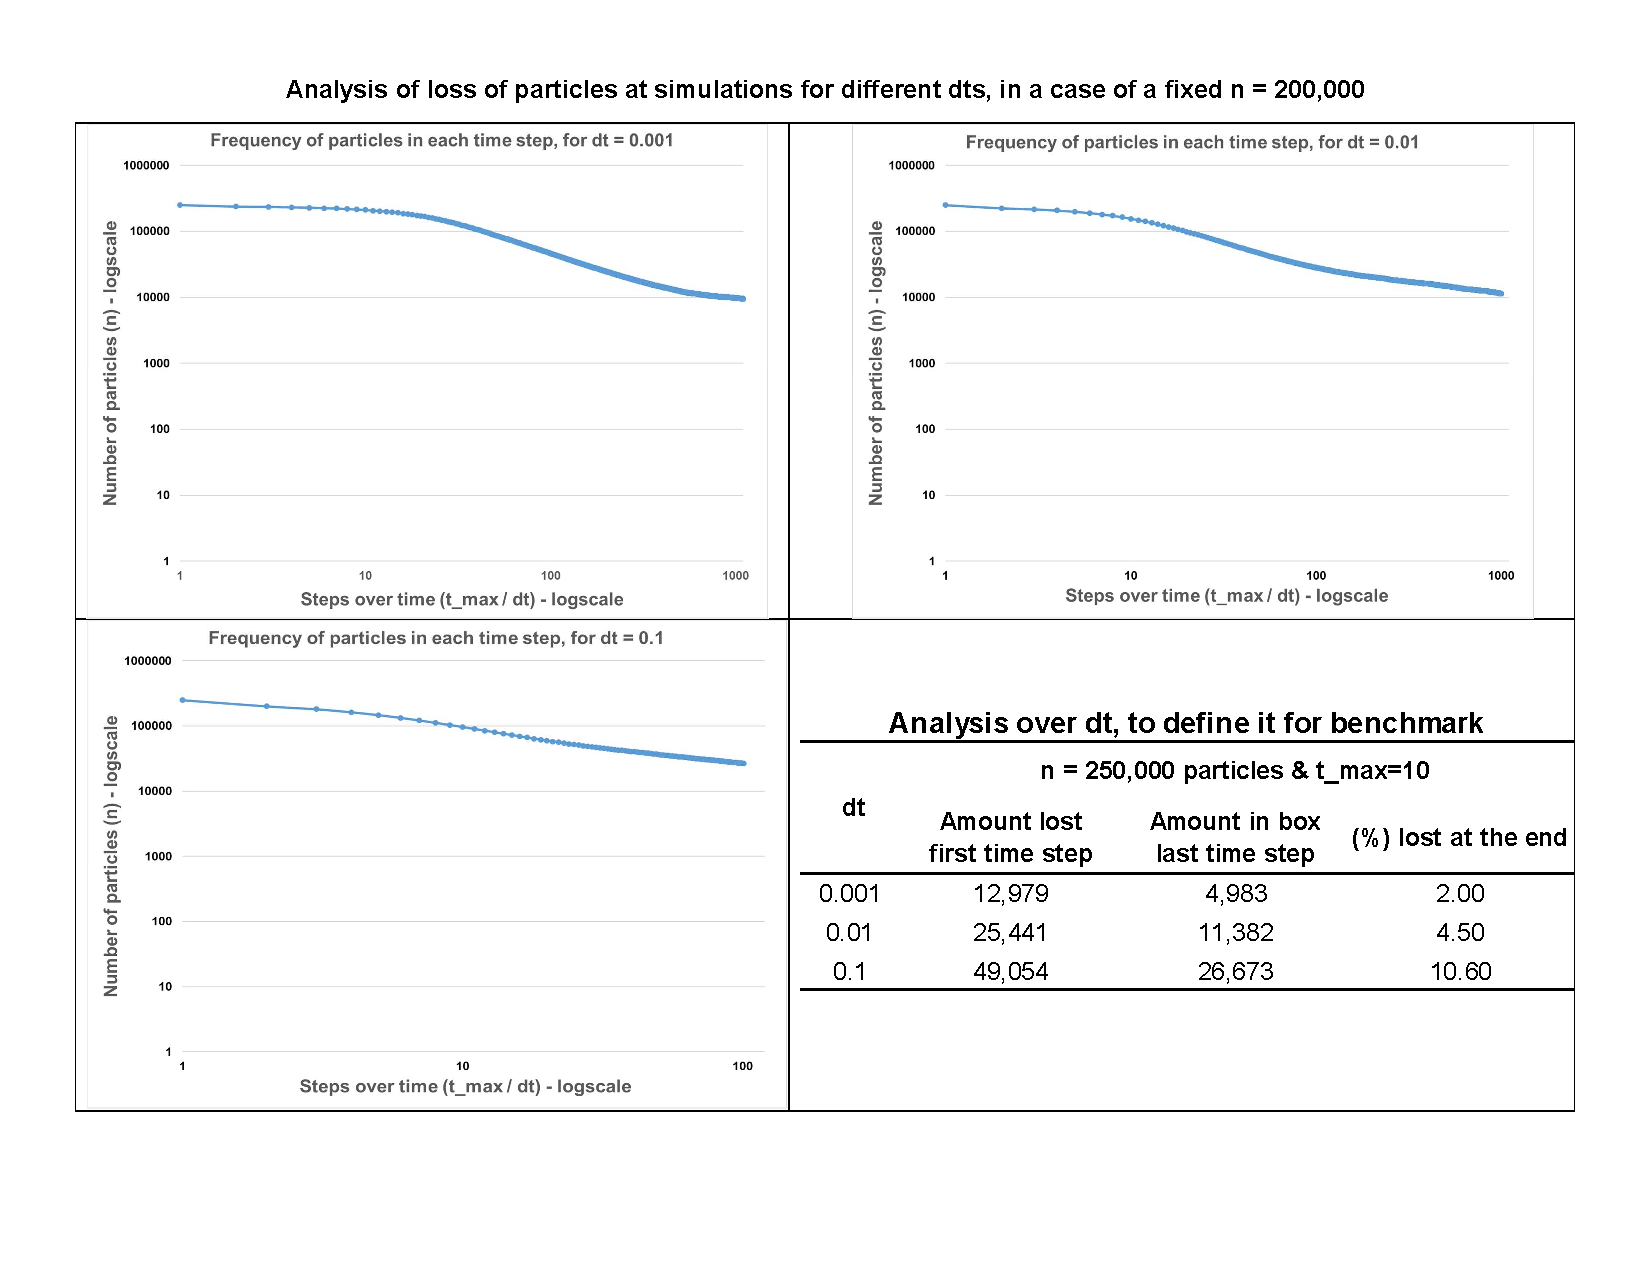
\includegraphics[width=0.75\textwidth]{Figures/PL.pdf}
		\caption{Comparison of number of particles lost for different time step sizes.}
		\label{fig:loss}
	\end{figure}
        
        For a fixed number of sectors, the wall times are expected to increase proportionally with respect to $N^2$. This behaviour was studied by fixing the number of sectors to 64 and varying the number of particles in the box. The results have been been presented in figure~\ref{fig:N_scaling}.
        	\begin{figure}[h]
		\centering
		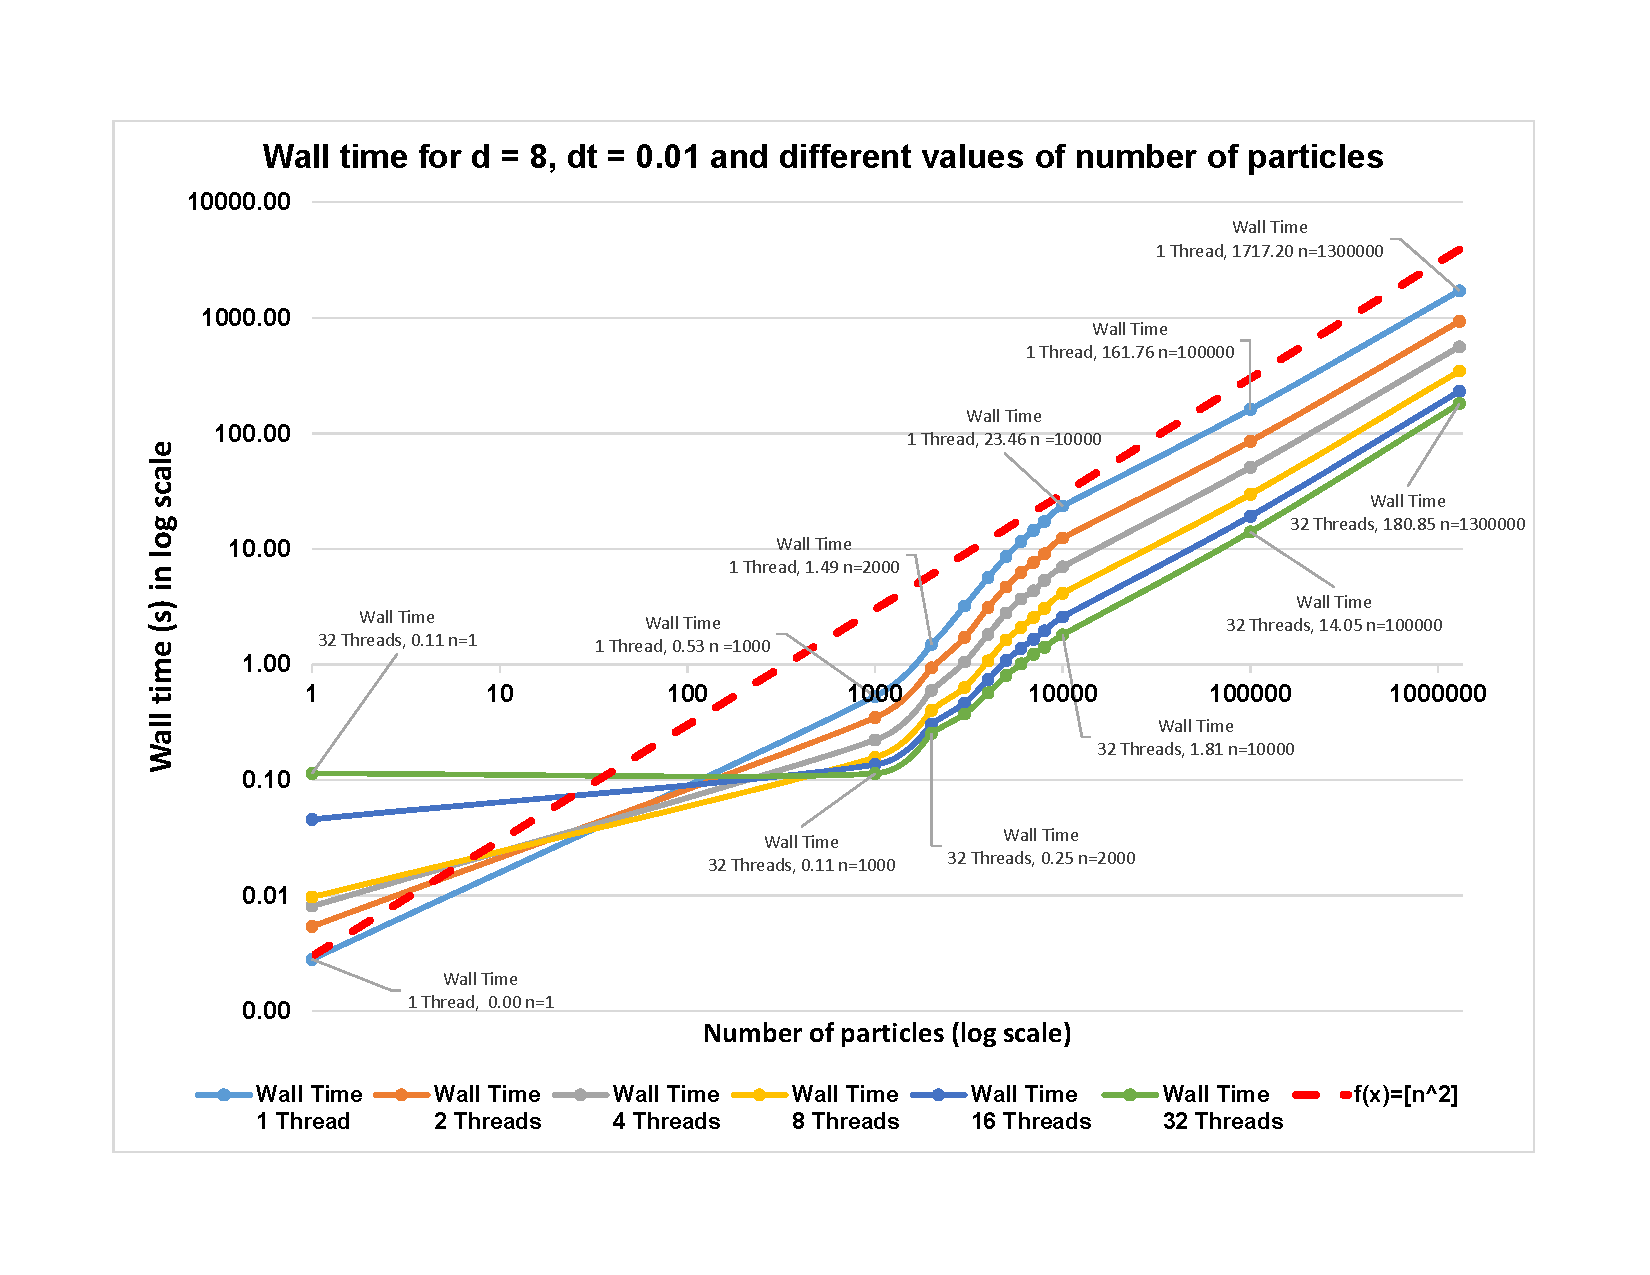
\includegraphics[width=0.75\textwidth]{Figures/N.pdf}
		\caption{Change in wallclock times for different number of particles.}
		\label{fig:N_scaling}
	        \end{figure}

       For a fixed number of particles, the wall times are expected to decrease proportionally with respect to $D^4$. This behaviour was studied by fixing the number of particles and varying the maximum number of rows/columns and has been presented in figure~\ref{fig:D_scaling}. While the behaviour is as expected for the initial part of the plot, we observe that after a certain number of sectors, as the number of sectors is further increased the wall times decrease at a reduced rate. This can be explained by increase in the overheads as the number of sectors is increased. The book-keeping costs, however, become significant only for a significantly large number of sectors as can be seen from the given plots. 
        	\begin{figure}[h]
		\centering
		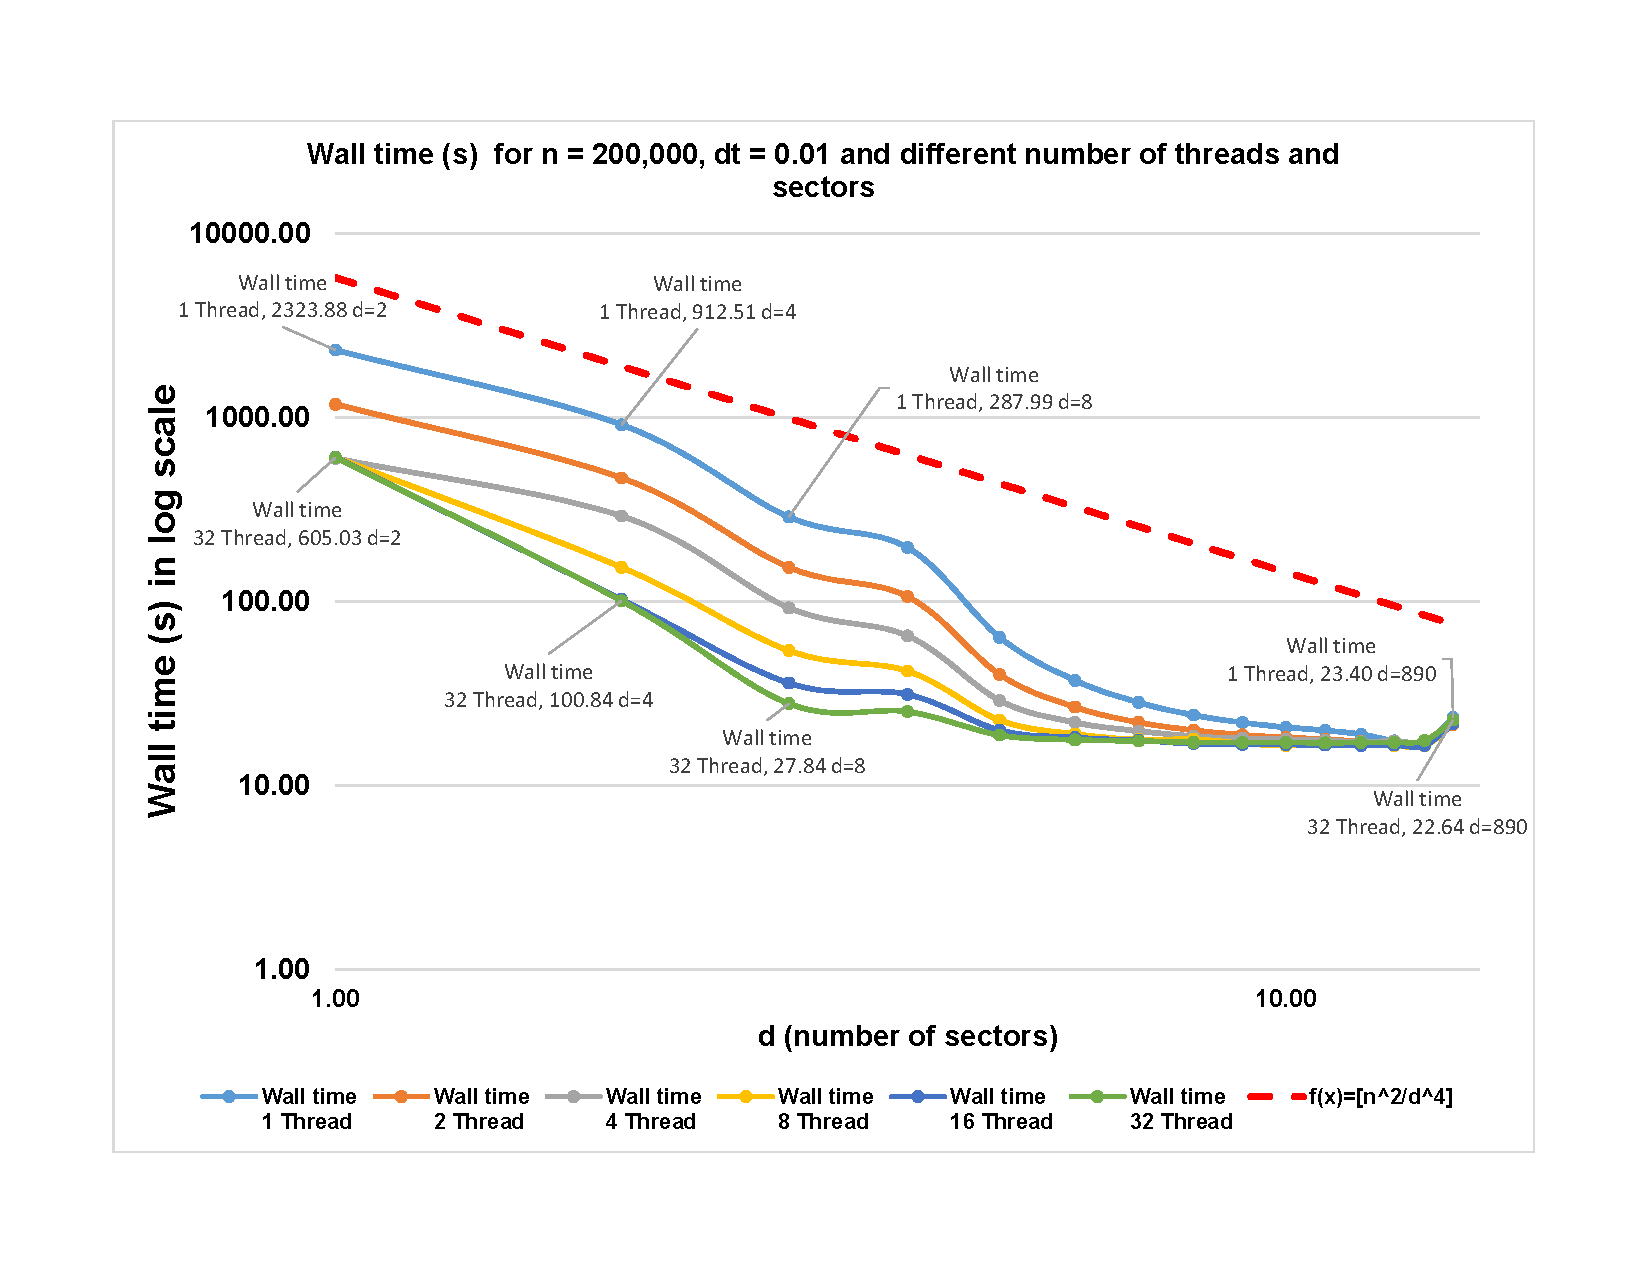
\includegraphics[width=0.75\textwidth]{Figures/D.pdf}
		\caption{Change in wallclock times for different number of sectors.}
		\label{fig:D_scaling}
	\end{figure}

                For a fixed value of number of particles $N$ and number of sectors $N^2$, the linear decrease in wallclock times with an increase in the number of threads has been presented in figure~\ref{fig:Threads}. While a reduction in wall times with increase in number of threads was observed for this case, the trend was not exactly linear. The speed-up and efficiency for the case have been presented in table~\ref{tab:measures}
	\begin{figure}[h]
		\centering
		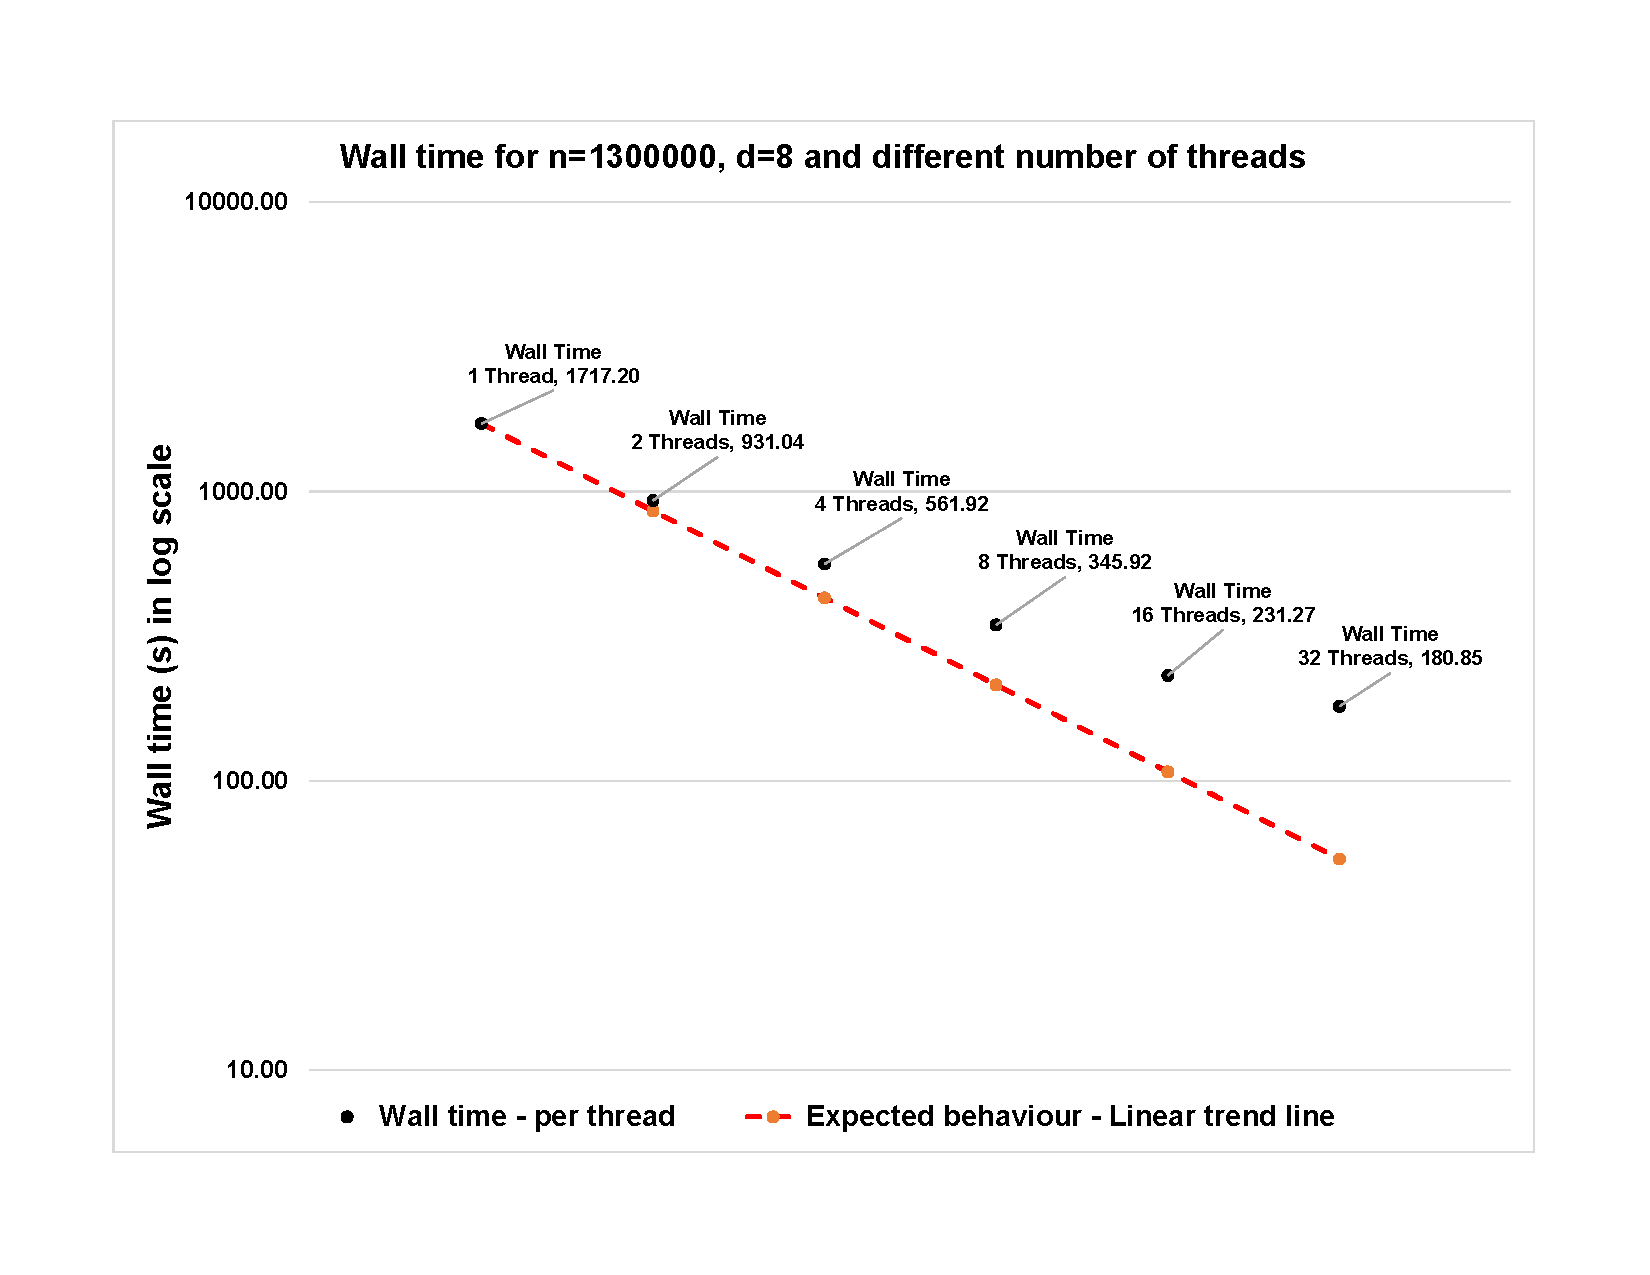
\includegraphics[width=0.75\textwidth]{Figures/Threads.pdf}
		\caption{Change in wallclock times for different number of threads.}
		\label{fig:Threads}
	\end{figure}
                
                \begin{table}[h]
  \caption{Speed-up and efficiency of parallelisation for $N = \num{1.3d6} \text{\&} D = 8$.}
  \label{tab:measures}
  \centering
  \begin{tabular}{ccccccc}
    \toprule
    \multirow{2}{*}{Number of Threads} &\phantom{abc} & \multirow{2}{*}{Wallclock Time [s]} &\phantom{abc} & \multicolumn{3}{c}{Parameter} \\
    \cmidrule{5-7}
    &\phantom{abc} & & \phantom{abc} & Speed-up & \phantom{abc} & {Efficiency}\\
    \midrule
    01 && 1717.20 && {} && {} \\
    02 && 931.04 && 1.84 && 0.92 \\
    04 && 561.92 && 3.06 && 0.76 \\
    08 && 345.92 && 4.96 && 0.62 \\
    16 && 231.27 && 7.42 && 0.46 \\
    32 && 180.85 && 9.50 && 0.30 \\
    \bottomrule
  \end{tabular}
\end{table}


\section{Conclusion}
     In conclusion, we can say that a number of physical and computational parameters affect the wall-clock times of the Langevin dynamics simulation. While the number of particles significantly impacts the wall-clock times, significant speed-ups can be obtained by domain discretisation and multi-threading. For a fixed number of particles, we observed that a minimum of 400 sectors with 2 threads gives an efficiency of at least 80\% and while we observe a continuous speed-up as the number of threads is increased, there is a loss of efficiency. With 32 threads, we found out that a minimum of 4000 particles were required to have an efficiency of 30\%.         

\bibliographystyle{ieeetr}
\bibliography{Assignment_2_Parikshit}

\end{document}  
